\section{Results and discussion} \label{sec:results_and_discussion}

In this report, the smartphone application proposed in \cite{sohappy} was 
implemented on Android, utilizing machine learning techniques in order to 
perform face and smile detection.

Since the app was primarily intended to be used in research, it was designed
with interchangeability in mind, allowing it to be used and adjusted as 
necessary in future studies. Especially with mental health being an important
topic amidst the current pandemic, the soHappy app can be used to aid research 
in affective computing.

soHappy is a tool enabling studies to motivate participants to smile on a 
regular basis. At the same time, the results are recorded and can be evaluated 
by researchers. Participating in such studies requires little effort from the 
users.

Regarding the soHappy smile detection machine learning model, the following
result is present: After the training is finished, it is evaluated with the
test data. As Figure \ref{fig:training_result} shows, the accuracy detecting a
smile as a smile is about 98\%, with an overall evaluation accuracy of about 
94.5\%.

\begin{figure}
  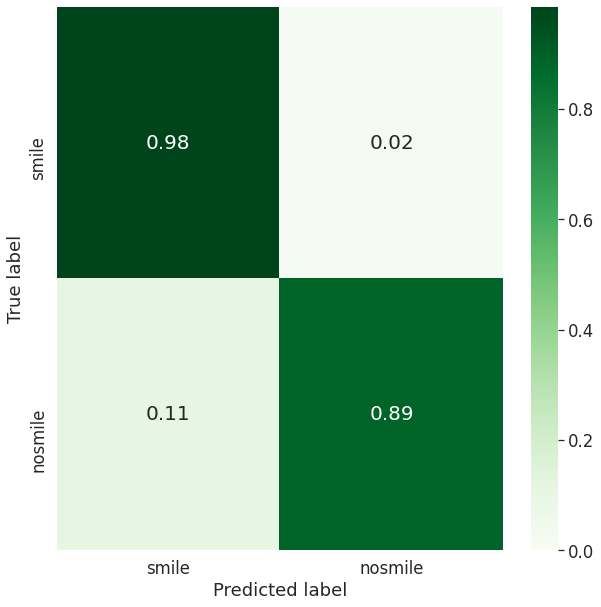
\includegraphics[width=\linewidth]{figures/training_result.png}
  \caption{Heatmap describing percentages of true-positives and true-negatives as well as false-negatives and false-positives.}
  \label{fig:training_result}
\end{figure}

While those numbers look promising, using this model in production shows
room for improvement. Sometimes it is not enough to smile with a closed
mouth. Instead, an open mouth is required.

In the future, the soHappy model could be improved by improving the machine 
learning architecture. Also, a bigger dataset including more photographs of
people smiling with their mouth closed could significantly increase 
performance.
